\documentclass[11pt]{beamer}
\usetheme{PaloAlto}

\usepackage[utf8]{inputenc}
\usepackage[T1]{fontenc}
\usepackage{amsmath}
\usepackage{amsfonts}
\usepackage{amssymb}
\usepackage{forest}
\usepackage{url}

\setbeamercolor{logo}{bg=white}

\author{Christoph Teichmann \and Antoine Venant}
\title{The Dirichlet Categorial Model}

\subtitle{}

\logo{\includegraphics[height=0.65cm]{SaarLogo}}

\institute{}

\date{}

\subject{}

\setbeamercovered{invisible}

\setbeamertemplate{navigation symbols}{}

\begin{document}
	
	\AtBeginSection[]{
		\begin{frame}
			\vfill
			\centering
			\begin{beamercolorbox}[sep=8pt,center,shadow=true,rounded=true]{title}
				\usebeamerfont{title}\insertsection\par%
			\end{beamercolorbox}
			\vfill
		\end{frame}
	}
	
	\begin{frame}
		\maketitle
	\end{frame}
	
	\section{Goals}
	
	\begin{frame}{Teaching Goals}
		\begin{itemize}
			\item Basic properties of Dirichlet Distribution
			\item Dirichlet Categorial Model
			\item Chinese Restaurant Process
			\item How to build a simple language model from that
		\end{itemize}
	\end{frame}
	
	\section{Motivation}
	
	\begin{frame}{Categorial Variables in Computationl Linguistics}
		\centering
		We want probabilites for random variables with discrete outcomes:
				
		\begin{itemize}
			\item Next word given previous ones
			\item Children given parent in binary constituent tree
			\item Next part-of-speech tag given previous ones
		\end{itemize}
		
		\vspace{20pt} Mary sees $\lbrace$ the, something, John, .\ $\rbrace$ \dots
	\end{frame}
	
	\begin{frame}{Categorial Variables in Computationl Linguistics}
		\centering
		We want probabilites for random variables with discrete outcomes:
		
		\begin{itemize}
			\item Next word given previous ones
			\item Children given parent in binary constituent tree
			\item Next part-of-speech tag given previous ones
		\end{itemize}
		
		\begin{tabular}{lr}
			\begin{forest}
				[S [ NP [Mary] ] [VP [ sees ] [NP [\dots] ] ] ]
			\end{forest} &
			\begin{tabular}{c}
				$NP \rightarrow something$ \\
				$NP \rightarrow John$
			\end{tabular}
		\end{tabular}
	\end{frame}
	
	\section{A Simple Approach}
	
	\begin{frame}{The Next Word -- The Bayesian Approach}
		\centering
		\begin{itemize}
			\item<1-> Find a dataset relevant to your problem
			\begin{itemize}
				\item<2-> sentences from websites (tokenized) \checkmark
			\end{itemize}
			\item<1-> Reduce your problem to estimating a random quantity of interest
			\begin{itemize}
				\item<3-> Probabilities for next word in context \checkmark 
			\end{itemize}
			\item<1-> Build joint probabilistic model of the data and the quantity to estimate
			\begin{itemize}
				\item<4-> uh oh
			\end{itemize}
		\end{itemize}
	\end{frame}
	
	\begin{frame}{Simple Model P(text|Probabilities)}
		\begin{itemize}
			\item N-Gram model
			\item $P(\overbrace{W_i}^{\text{random variable for word}}|\overbrace{w_{i-1}}^{\text{concrete value for word}},\dots,w_{0}) = P(W_i|w_{i-1},\dots,w_{i-(n-1)})$
			\item let us start with $n=1$, i.e., Unigram Model: $P(W_i|w_{i-1},\dots,w_{0}) = P(W_i)$ 
		\end{itemize}
		
		\vspace{10pt}Model for data given word probabilities -- where to get word probabilities?
	\end{frame}
	
	\begin{frame}{Simplest Choice -- How to Write Word Probabilities}
		\begin{itemize}
			\item Assume finite lexicon $L$
			\item Probability word is ``Mary''  $P(W = \text{Mary})$
			\item Random variable over distributions $P^X$, $P^x$ single distribution
			\item Full joint model $P\left( P^{X},W_1,\dots,W_n \right)$
		\end{itemize}
	\end{frame}
	
	\begin{frame}{Simplest Choice -- Everything Equally Likely}
		\begin{itemize}
			\item Let us start with an uniform model, i.e.\ $P\left( P^X = P^{x} \right) = \frac{1}{Z}$
			\item $Z$ is a constant to ensure integration to $1$
			\item We think $P^{x}(the) = 0.9$ is as likely as any other value
		\end{itemize}
		
		\vspace{10pt}Similar to model from last session
	\end{frame}
	
	\begin{frame}{How Does This Work}
		\begin{itemize}
			\item Lexicon: $L = \lbrace \text{Mary}, \text{sees}, \text{.}, \text{something}, \text{John}  \rbrace$
			\item Dataset: $D=$``Mary sees something''
			\item What is the Posterior, i.e., what is $P(P^x | \text{something},\text{sees},\text{Mary})$ for a given $P^x$
			\item What is the next word? (hint: ``.'')
		\end{itemize}
	\end{frame}
	
	\begin{frame}{Posterior}		
		\begin{align*}
			\overbrace{P(P^X = P^x \vert w_3,w_2,w_1)}^{\text{Posterior}} & \sim \left(\overbrace{\prod_{i \in \{1,2,3\}} P^{X}(w_i)}^{\text{Word Model}}\right) \overbrace{\frac{1}{Z}}^{\text{Prior}}
		\end{align*}
		
		\vspace{10pt} Is this (proportional to) a known distribution?
	\end{frame}
	
	\section{The Dirichlet Distribution}
	
	\begin{frame}{Is This A Known Distribution?}
		Dirichlet Distribution -- distribution over probability distributions $P^x$ with outcomes $o_1,\dots,o_k$:
		
		\begin{align*}
			P_{Dir}(P^x) & = \frac{\prod_{i \in [1,K]} P^{x}(o_i)^{\alpha_i}}{B(\boldsymbol{\alpha})}
		\end{align*}
		
		\vspace{10pt} \begin{itemize}
			\item Here	$\alpha_i > 0$ are parameters -- there are lots of Dirichlet Distributions
			\item $B(\boldsymbol{\alpha})$ is a normalizer depending on all the $a_i$ -- look it up on Wikipedia
		\end{itemize}
	\end{frame}
	
	\begin{frame}{It is a Dirichlet Distribution!}
		\begin{align*}
			P_{Dir}(P^X) & = \frac{\prod_{i \in [1,K]} P^{x}(o_i)^{\alpha_i}}{B(\boldsymbol{\alpha})} \\
			P(P^x \vert w_3,w_2,w_1) & \sim \left(\prod_{i \in \{1,2,3\}} P^{x}(w_i)\right) \frac{1}{Z} \\
			& \sim \frac{\prod_{w \in L} P{x}(w)^{\sum_{i \in [1,3]} 1(w_i = w)}}{Z}
		\end{align*}
		
		\vspace{10pt}\begin{itemize}
			\item Here the $\alpha$s correspond to counts of how often we have seen each word $+1$
			\item Note that the uniform distribution over probability distributions is the same as the Dirichlet Distribution with $\boldsymbol{\alpha} = \boldsymbol{1}$ 
		\end{itemize}
	\end{frame}
	
	\begin{frame}{Visualizing a Dirichlet Distribution With Two Outcomes}
		\begin{center}
			\includegraphics[width=0.75\linewidth]{dirichlet_distribution_pdf}
		\end{center}
		
		\begin{tiny}
			Generated with code based on code found at: \url{https://commons.wikimedia.org/wiki/File:Beta_distribution_pdf.svg} by user Horas based on the work of user Krishnavedala
		\end{tiny}
	\end{frame}
		
	\begin{frame}{Understanding the Behaviour of the Dirichlet}
		\begin{itemize}
			\item Increase $\alpha$s $\rightarrow$ concentrates at values proportional to $\alpha$s
			\item If all $\alpha$ are less than 1, then we favour ``sparse distributions'' few outcomes likely
		\end{itemize}
		
		\begin{tabular}{lr}
			\includegraphics[width=0.49\linewidth]{dirichlet_distribution_sparse_pdf} &
			\includegraphics[width=0.49\linewidth]{dirichlet_distribution_dense_pdf} \\
		\end{tabular}
	\end{frame}
		
	\begin{frame}{Back to the Example}
		For our example our posterior is:

		\vspace{10pt}		
		\begin{align*}
			P(P^x) & = \frac{\left(\prod_{w \in L} P^{x}(w)^{\alpha_{w_i}}\right)}{B(\boldsymbol{\alpha})}
		\end{align*}
		
		\vspace{10pt} Where $\alpha_{\text{Mary}}=\alpha_{\text{sees}} = \alpha_{\text{something}} = 2$ and $\alpha_{\text{John}}=\alpha_{\text{.}}=1$
	\end{frame}
	
	\begin{frame}{What We Have}
		\begin{itemize}
			\item We now have a posterior probability for the different $P_{w}^{x}$ and know it is a Dirichlet Distribution
			\item What are the probabilities for the next word -- what is the predictive distribution?
		\end{itemize}
	\end{frame}
	
	\begin{frame}{Predictive Distribution}
		\begin{align*}
			P(W_4 = w_4) = \int_{P^x} P^x(w_4) \frac{\left(\prod_{w \in L} P^{x}(w)^{\alpha_{w}}\right)}{B(\boldsymbol{\alpha})} d P^x
		\end{align*}
		
		\vspace{10pt} Let us just look it up, e.g., the Dirichlet write up at \url{https://people.eecs.berkeley.edu/~stephentu/} 
	\end{frame}
	
	\begin{frame}{Predictive Distribution}
		\begin{align*}
			P(W_4 = w_4) & = \int_{P^x} P^x(w_4) \frac{\left(\prod_{w \in L} P^{x}(w)^{\alpha_{w}}\right)}{B(\boldsymbol{\alpha})} d P^x \\
			P(W_4 = w_4) & = \frac{\alpha_{w_4}}{\sum_{w \in L} \alpha_{w}}
		\end{align*}
			
		\vspace{10pt}
		\begin{itemize}
			\item Likelihood of outcome is $\alpha$ for that outcome divided by sum of $\alpha$s for all outcomes (finish example on table)
			\item This model is called a \textbf{Dirichlet Categorial Distribution}
		\end{itemize}
		 
	\end{frame}
	
	\begin{frame}{The Next Word -- The Bayesian Approach}
		\centering
		\begin{itemize}
			\item Find a dataset relevant to your problem
			\begin{itemize}
				\item sentences from websites (tokenized) \checkmark
			\end{itemize}
			\item Reduce your problem to estimating a random quantity of interest
			\begin{itemize}
				\item Probabilities for next word in context \checkmark 
			\end{itemize}
			\item Build joint probabilistic model of the data and the quantity to estimate
			\begin{itemize}
				\item Unigram model with uniform prior \checkmark
			\end{itemize}
			\item<2-> Get a posterior distribution
			\begin{itemize}
				\item<2-> We get a Dirichlet Distribution posterior, which is well understood \checkmark
				\item<2-> We can predict the next word using knowledge about Dirichlet Categorial Model \checkmark
			\end{itemize}
			\item<3-> Check model quality and revise if necessary
		\end{itemize}
	\end{frame}
	
	\begin{frame}{Is Our Model Reasonable?}
		Predictive probabilities for any word position:
		
		\begin{align}
			P(W_4 = \text{.}) & = \frac{1}{8} \\
			P(W_4 = \text{Mary}) & = \frac{2}{8}
		\end{align}
		
		\vspace{10pt}Data may support this, but it seems unlikely given what we know about English
	\end{frame}
	
	\begin{frame}{A Better Model}
		\begin{itemize}
			\item We assumed that we have unigram word probabilities -- switch to e.g.\ a bigram model
			\item Instead of assuming uniform probability for different $P^{x}$ we could assume Dirichlet Prior with different $\alpha$s
		\end{itemize}
	\end{frame}
	
	\begin{frame}{New Model}
		\begin{itemize}
			\item<1-> We now have to find probabilities $P^{x}(W_i = w_i|w_{i-1})$
			\item<1-> For each we will have a Dirichlet Prior with $\alpha$s proportional to observed word frequencies in some corpus
			\item<2-> Let us work through that for the data:
				\begin{itemize}
					\item<2-> ``Mary saw something .''
					\item<2-> ``John saw''
				\end{itemize}
		\end{itemize}
	\end{frame}
	
	\begin{frame}{Conjugate Model}
		What is the general posterior with the Dirichlet model after words $w_1,\dots,w_n$?
		
		\begin{align}
			P(P^{x}) & = \frac{\prod_{w \in L} P^{x}(w)^{\alpha_{w}+\sum_{i \in [1,n]} 1(w_i = w)}}{Z}
		\end{align}			
		
		\begin{itemize}
			\item Another Dirichlet Distribution
			\item If prior and piosterior are same type $\rightarrow$ conjugate model
			\item helpful because understanding the prior means you understand the posterior
		\end{itemize}
	\end{frame}
	
	\begin{frame}{The Next Word -- The Bayesian Approach}
		\centering
		\begin{itemize}
			\item Find a dataset relevant to your problem
			\begin{itemize}
				\item sentences from websites (tokenized) \checkmark
			\end{itemize}
			\item Reduce your problem to estimating a random quantity of interest
			\begin{itemize}
				\item Probabilities for next word in context \checkmark 
			\end{itemize}
			\item Build joint probabilistic model of the data and the quantity to estimate
			\begin{itemize}
				\item unigram model with uniform prior \checkmark
			\end{itemize}
			\item Get a posterior distribution
			\begin{itemize}
				\item We get a Dirichlet Distribution posterior, which is well understood \checkmark
				\item We can predict the next word using knowledge about Dirichlet Categorial model \checkmark
			\end{itemize}
			\item Check model quality and revise if necessary
			\begin{itemize}
				\item Larger n-grams with better prior \checkmark
			\end{itemize}
		\end{itemize}
	\end{frame}
	
	\section{The Dirichlet Process}
	
	\begin{frame}{Further Model Problems}
		``Mary saw a cake .''
		
		\vspace{10pt}Probably more than 5 words in English
	\end{frame}
	
	\begin{frame}{Moving to the Dirichlet Process}
		
		\begin{itemize}
			\item $P(X)$ single outcome probability distribution
			\item $P(X_1,\dots,X_n)$ $\rightarrow$ multiple outcome probability distribution
			\item $P(X_1,X_2,X_3\dots)$ $\rightarrow$ stochastic process / random function
		\end{itemize}
	\end{frame}
	
	\begin{frame}{Extension to Infinite Number of Variables}
		\begin{itemize}
			\item Use what we know about Dirichlet Distribution
			\item How can we define an infinite list of $\alpha$s?
			\item How to define a process?
		\end{itemize}
	\end{frame}
	
	\begin{frame}{How Can We Define an Infinite List of $\alpha$s?}
		\centering
		
		\begin{itemize}
			\item When you have a hammer $\dots$
			\item Define a single concentration parameter $\alpha$ and a \text{base} probability distribution (measure) $P(X)$
			\item $\alpha_x = \alpha P(X = x)$
			\item different $\alpha$s always sum to concentration parameter
		\end{itemize}
		
		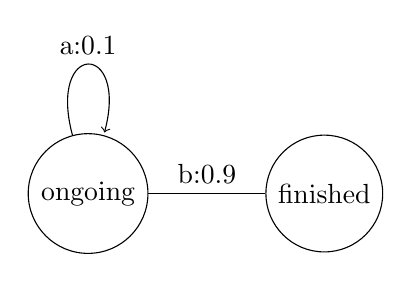
\begin{tikzpicture}
			\node[draw,circle] (1) at (0,0) {ongoing};
			\node[draw,circle] (2) at (3,0) {finished};
			
			\path
			(1) edge [loop above] node {a:0.1} (1);
			\path (1) edge node [above] {b:0.9} (2);
		\end{tikzpicture}
		
		\vspace{10pt} If $\alpha = 10$ what is $\alpha_{\text{ab}}$?
	\end{frame}
	
	\begin{frame}{Extension to Infinite Number of Variables}
		\begin{itemize}
			\item How can we define an infinite list of $\alpha$s?
			\begin{itemize}
				\item Concentration parameter + probability distribution \checkmark
			\end{itemize}
			\item How to define a process?
		\end{itemize}
	\end{frame}
	
	\begin{frame}{How to Define a Process}
		\begin{itemize}
			\item No need to define probability for a full outcome $P(X_1=x_1,X_2=x_2,\dots)$
			\item If we pick a few values for a few variables and do not care about all the others -- what is the probability?
			\item Probability Distributions for any $X^1,X^2,\dots,X^m$ follow a Dirichlet
		\end{itemize}
	\end{frame}
	
	\begin{frame}{Making it Concrete}
		\centering
		
		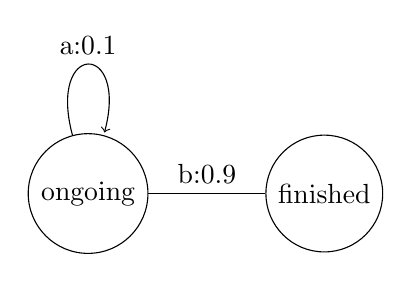
\begin{tikzpicture}
			\node[draw,circle] (1) at (0,0) {ongoing};
			\node[draw,circle] (2) at (3,0) {finished};
		
			\path
			(1) edge [loop above] node {a:0.1} (1);
			\path (1) edge node [above] {b:0.9} (2);
		\end{tikzpicture}
		
		\begin{align*}
			P_{Dir}(P_X) & = \frac{\prod_{i \in [1,K]} P_{X}(o_i)^{\alpha_i}}{B(\boldsymbol{\alpha})} \\
			\alpha = 10
		\end{align*}
		
		\begin{align*}
		P(P^x(b) = 0.2,P^x_(ab) = 0.5) & = &
		\frac{\overbrace{0.2^{9}}^{b} \times \overbrace{0.5^{0.9}}^{ab} \times
			\overbrace{0.3^{0.1}}^{\text{everything else}}}{B(\langle 9,0.9,0.1 \rangle)}
		\end{align*}
	\end{frame}
	
	\begin{frame}{Extension to Infinite Number of Variables}
		\begin{itemize}
			\item How can we define an infinite list of $\alpha$s?
			\begin{itemize}
				\item Concentration parameter + probability distribution \checkmark
			\end{itemize}
			\item How to define a process?
			\begin{itemize}
				\item Define probability distribution for any finite selection of variables
			\end{itemize}
		\end{itemize}
	\end{frame}
	
	\begin{frame}{Applying for Next Word Prediction}
		\begin{itemize}
			\item Bigram Model
			\item Infinitely many possible words $w_i$
			\item Probabilities for each $P(W_i|w_{i-1},w_{i-2})$ come from Dirichlet Process
			\item Pick some concentration parameter $\alpha$
			\item use a HMM over Morphems to define base probabilities $P(X)$
		\end{itemize}
		
		\vspace{10pt} What is the predictive density / what is the posterior?
	\end{frame}
	
	\begin{frame}{Predictive Density}
		Still a Dirichlet Categorical Distribution!
		
		\begin{align*}
			P(W_{0}=ab) = \frac{\alpha_{ab}}{\alpha}
		\end{align*}
	\end{frame}
	
	\begin{frame}{Posterior}
		Still a Dirichlet Process!
		
		\vspace{10pt} Seen ``ab'' as first word - now $\alpha_{ab}' = \alpha_{ab}+1$, $\alpha' = \alpha + 1$ 
	\end{frame}
	
	\section{Chinese Restaurant Process}
	
	\begin{frame}{Can We Make This Simpler?}
		\begin{itemize}
			\item Chinese Restaurant Process -- metaphor for Dirichlet Categorial Model
			\item Every word is a table
			\item Number of people at table $x$ is $\alpha_x$
			\item People are likely to sit at popular tables
		\end{itemize}
	\end{frame}
	
	\begin{frame}{Example}
		\centering
		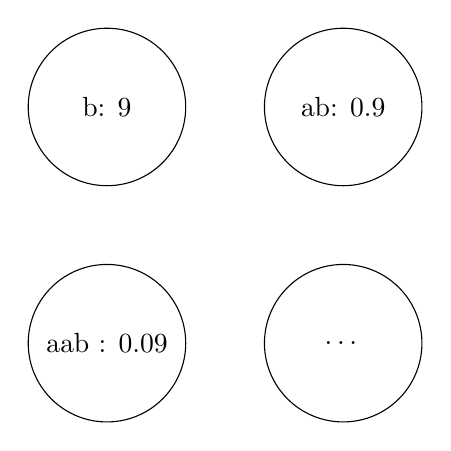
\begin{tikzpicture}
			\node[draw,circle,minimum size=2cm] (b) at (0,0) {b: 9};
			\node[draw,circle,minimum size=2cm] (ab) at (3,0) {ab: 0.9};
			\node[draw,circle,minimum size=2cm] (aab) at (0,-3) {aab : 0.09};
			\node[draw,circle,minimum size=2cm] (dots) at (3,-3) {\dots};
		\end{tikzpicture}
		
		\vspace{10pt} Chance the first costumer sits at ``b'' $\frac{9}{10}$
	\end{frame}
	
	\begin{frame}{Example}
		\centering
		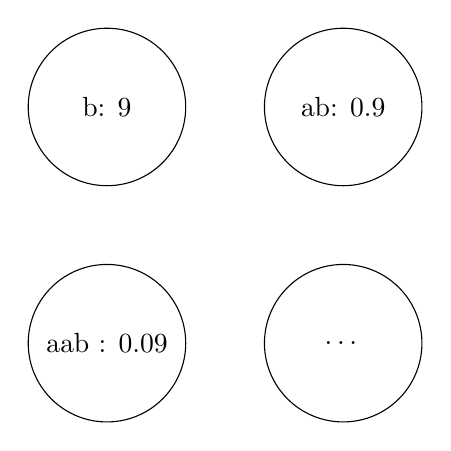
\begin{tikzpicture}
		\node[draw,circle,minimum size=2cm] (b) at (0,0) {b: 9};
		\node[draw,circle,minimum size=2cm] (ab) at (3,0) {ab: 0.9};
		\node[draw,circle,minimum size=2cm] (aab) at (0,-3) {aab : 0.09};
		\node[draw,circle,minimum size=2cm] (dots) at (3,-3) {\dots};
		\end{tikzpicture}
		
		\vspace{10pt} Chance the first costumer sits at ``ab'' $\frac{0.9}{10}$
	\end{frame}
	
	\begin{frame}{Example}
		\centering
		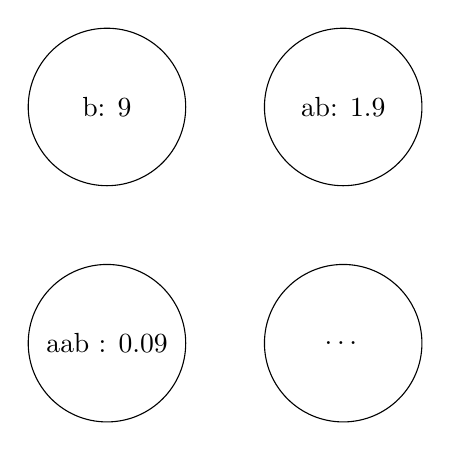
\begin{tikzpicture}
		\node[draw,circle,minimum size=2cm] (b) at (0,0) {b: 9};
		\node[draw,circle,minimum size=2cm] (ab) at (3,0) {ab: 1.9};
		\node[draw,circle,minimum size=2cm] (aab) at (0,-3) {aab : 0.09};
		\node[draw,circle,minimum size=2cm] (dots) at (3,-3) {\dots};
		\end{tikzpicture}
		
		\vspace{10pt} First costumer sits at ``ab''
		
		\vspace{10pt} Chance the second costumer sits at ``ab'' $\frac{1.9}{11}$
	\end{frame}
	
	\begin{frame}{Presentation in Papers}
		\begin{itemize}
			\item Usual presentation: tables are created when first costumer sits at them
			\item New table created with $\frac{\alpha}{\alpha+\text{seen}}$
			\item New table label -- according to base probability distribution
			\item  Sitting at old table $\frac{\text{costumers old table}}{\alpha+\text{seen}}$
		\end{itemize}
	\end{frame}
	
	\section{Summary}
	
	\begin{frame}{Take Away}
		\begin{itemize}
			\item Important for NLP: categorial probability distributions
			\item Handy prior: Dirichlet Distribution/Process
			\item Works for infinite choices as well
			\item Posterior is also Dirichlet Distribution/Process
			\item Predictive distribution easy to read off $\alpha$
			\item Chinese Restaurant metaphor used frequently
		\end{itemize}
	\end{frame}
	
	\begin{frame}
		\centering
		\begin{Large}
			\textbf{Questions!}
		\end{Large}
	\end{frame}
	
\end{document}